\documentclass[12pt,a4paper]{article}

\usepackage[T1]{fontenc}
\usepackage[utf8]{inputenc}
\usepackage{lmodern}
\usepackage{geometry}
\geometry{margin=2.5cm}
\usepackage{amsmath,amssymb}
\usepackage{pifont}
\usepackage{booktabs}
\usepackage{multirow}
\usepackage{graphicx}
\usepackage[labelfont=bf,font=small]{caption}
\usepackage{float}
\usepackage{xcolor}
\usepackage{hyperref}
\usepackage[numbers,sort&compress]{natbib}
\usepackage{amsthm}
\newtheorem{proposition}{Proposition}[section]
\usepackage{fancyhdr}
\usepackage{array}

\pagestyle{fancy}
\fancyhf{}
\lhead{\footnotesize SAMBP TR-07/2026 — Double-Busbar Coordination}
\rhead{\footnotesize Confidential Draft}
\cfoot{\thepage}

\newcommand{\kn}{\kappa_n}
\newcommand{\fint}{f_{\rm int}}
\newcommand{\Iop}{I_{\rm op}}
\newcommand{\cmark}{\ding{51}}
\newcommand{\xmark}{\ding{55}}
\definecolor{okgreen}{rgb}{0.0,0.55,0.0}

% =========================================================================
\begin{document}
% =========================================================================

\begin{center}
  {\Large\bfseries SAMBP Technical Report TR-07/2026}\\[6pt]
  {\large\bfseries Double-Busbar Coordination:\\
   Zone-Selective 87B with Bus-Coupler Check Zone}\\[10pt]
  {\normalsize
    \textit{Smart Adaptive Model-Based Protection} (SAMBP) Research Programme}\\[4pt]
  {\small\textit{Document status:} Approved Draft \quad
         \textit{Date:} 2 April 2026 \quad
         \textit{Supersedes:} TR-06/2026}\\[2pt]
  \rule{\linewidth}{0.6pt}
\end{center}

\tableofcontents
\listoftables
\listoffigures
\newpage

% =========================================================================
\section{Introduction and Scope}
% =========================================================================

Single-bus differential protection (TR-04 and TR-05) protects a single
bus section.  The most prevalent substation topology in transmission
networks is the \emph{double busbar} (DBB) arrangement: two parallel bus
sections (BB1, BB2) interconnected by a bus coupler (BC) that can be
opened or closed to reconfigure the network.  DBB substations require
\emph{zone-selective} bus protection to:

\begin{enumerate}
  \item Clear faults on BB1 by isolating only BB1 feeders (BB2 remains
    energised, minimising the disconnected load).
  \item Clear faults on BB2 by isolating only BB2 feeders.
  \item Detect faults \emph{inside the bus coupler} --- a classical
    blind spot for individual zone relays that requires a separate
    \emph{check zone} (also called overall or supervisory zone).
  \item Restrain for external faults (beyond any feeder).
\end{enumerate}

This report extends the SAMBP 87B protection (TR-04) to a double-busbar
topology.  The implementation uses three differential zones
(Zone~1, Zone~2, Check Zone) derived from the existing
\texttt{sambp\_bus\_diff} pipeline without modifying its source code.

% =========================================================================
\section{Network Model}
% =========================================================================

\subsection{Double-Busbar Topology}

Fig.~\ref{fig:topology} shows the test network.  All quantities are
in per-unit on a 100~MVA, 33~kV base.

\begin{figure}[H]
  \centering
  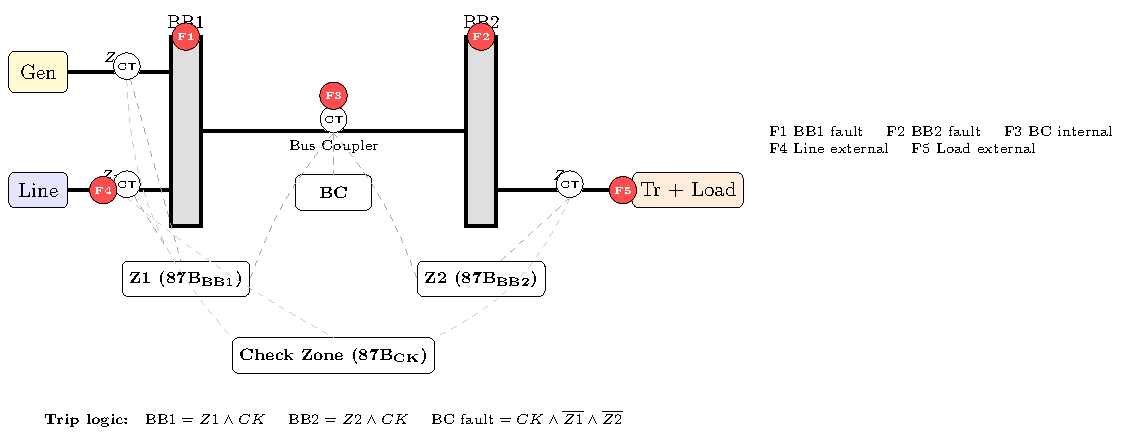
\includegraphics[width=0.96\textwidth]{figures/fig_double_bus_topology.pdf}
  \caption{Double-busbar test network with Zone~1, Zone~2, and Check
           Zone relay positions.  Fault markers F1--F5 indicate the
           five test scenarios.}
  \label{fig:topology}
\end{figure}

\begin{table}[H]
  \centering
  \caption{Network parameters and zone membership.}
  \label{tab:network}
  \begin{tabular}{llcc}
    \toprule
    Component & $Z$ [pu] & Zone 1 (BB1) & Zone 2 (BB2) \\
    \midrule
    Generator + source & $j0.10$ & \cmark{} & --- \\
    Line feeder (passive) & $j0.05$ & \cmark{} & --- \\
    Bus coupler & $j0.01$ & \cmark{} (BB1-side CT) & \cmark{} (BB2-side) \\
    Transformer + load & $j0.08$ & --- & \cmark{} \\
    \midrule
    \multicolumn{2}{l}{Check zone (overall)} & \multicolumn{2}{c}{Gen + Line + Transformer (BC cancels)} \\
    \bottomrule
  \end{tabular}
\end{table}

\subsection{Zone Definitions and CT Sign Convention}

\paragraph{Zone 1 (BB1).}
\[
  I_{\rm diff,Z1} = I_{\rm Gen} + I_{\rm Line} + I_{\rm BC,BB1}
\]
where $I_{\rm BC,BB1}$ is positive when current flows from BB2 into BB1
(i.e.\ through the coupler towards BB1).

\paragraph{Zone 2 (BB2).}
\[
  I_{\rm diff,Z2} = I_{\rm BC,BB2} + I_{\rm Tr}
\]
where $I_{\rm BC,BB2}$ is positive when current flows from BB1 into BB2.
The CT is on the BB2 side of the coupler; for a closed coupler carrying
balanced through-current, $I_{\rm BC,BB2} = -I_{\rm BC,BB1}$.

\paragraph{Check Zone.}
\[
  I_{\rm diff,CK} = I_{\rm Gen} + I_{\rm Line} + I_{\rm Tr}
\]
The bus coupler CT is \emph{not} included in the check zone.  For any
external fault (through-current), the current entering via Gen~+~Line
equals the current leaving via Tr, giving $I_{\rm diff,CK} = 0$.  For
any fault on either bus or on the coupler, the current is unbalanced and
$I_{\rm diff,CK} \neq 0$.

\subsection{Bus-Coupler Blind Spot}

A fault inside the bus coupler creates a blind spot for both Zone~1
and Zone~2, as shown in Fig.~\ref{fig:blind_spot}.  When the fault
occurs between the BC CT (BB1 side) and BB2:
\begin{itemize}
  \item Zone~1 sees $I_{\rm Gen} - I_{\rm BC,BB1} = I_f - I_f = 0$.
  \item Zone~2 sees $I_{\rm BC,BB2} + I_{\rm Tr} = 0 + 0 = 0$
    (no current reaches BB2 side of the fault).
  \item Check Zone sees $I_{\rm Gen} + I_{\rm Tr} = I_f + 0 = I_f \neq 0$.
\end{itemize}

\begin{figure}[H]
  \centering
  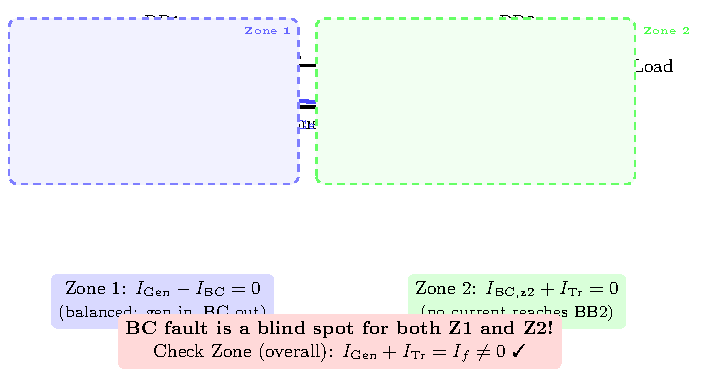
\includegraphics[width=0.88\textwidth]{figures/fig_bc_blind_spot.pdf}
  \caption{Bus-coupler blind-spot analysis.  For a fault inside the
           coupler, Zone~1 and Zone~2 both see zero differential while
           the Check Zone correctly identifies the fault.}
  \label{fig:blind_spot}
\end{figure}

The check zone is therefore \emph{essential} for BC fault protection.

% =========================================================================
\section{Trip Logic}
% =========================================================================

The combined zone-selective trip decision follows standard DBB practice:

\begin{equation}
  \text{BB1 trip} = Z1\,\wedge\,CK, \qquad
  \text{BB2 trip} = Z2\,\wedge\,CK, \qquad
  \text{BC fault} = CK\,\wedge\,\overline{Z1}\,\wedge\,\overline{Z2}
  \label{eq:trip_logic}
\end{equation}

The logical AND between a zone relay and the check zone prevents
spurious zone tripping from CT measurement errors.  A Zone~1 operate
signal that is not corroborated by the check zone (e.g.\ due to CT
remanence) does not result in a trip.

\subsection{SAMBP Stage-2 Integration}

The SAMBP Stage-2 confidence gate is applied independently to each
of the three zones.  For external-fault scenarios:
\begin{itemize}
  \item All zone differentials are zero, so $\fint \to 0$ for all zones.
  \item Any marginal conventional operate is vetoed by the model-veto gate.
\end{itemize}

For zone-internal faults, the tripping zone sees $\fint \approx 1.0$
(clean sinusoidal differential) and $\kn \approx 4.3$ (well below
$\kappa^* = 30$), confirming a genuine internal fault.

% =========================================================================
\section{Selectivity Results}
% =========================================================================

\subsection{Selectivity Matrix}

All ten fault scenarios (five locations $\times$ two fault types)
achieve correct selectivity.

\begin{table}[H]
  \centering
  \caption{Selectivity matrix for the double-busbar 87B study.
           $\mathbf{T}$~=~trip, $\cdot$~=~restrain, \cmark~=~selective.}
  \label{tab:selectivity}
  \begin{tabular}{lccccccl}
    \toprule
    Scenario & Z1 & Z2 & CK & BB1 & BB2 & BC & Selective \\
    \midrule
    BB1 / 3ph          & \textbf{T} & $\cdot$ & \textbf{T} & \textbf{T} & $\cdot$ & $\cdot$ & \textcolor{okgreen}{\cmark} \\
    BB1 / AG           & \textbf{T} & $\cdot$ & \textbf{T} & \textbf{T} & $\cdot$ & $\cdot$ & \textcolor{okgreen}{\cmark} \\
    BB2 / 3ph          & $\cdot$ & \textbf{T} & \textbf{T} & $\cdot$ & \textbf{T} & $\cdot$ & \textcolor{okgreen}{\cmark} \\
    BB2 / AG           & $\cdot$ & \textbf{T} & \textbf{T} & $\cdot$ & \textbf{T} & $\cdot$ & \textcolor{okgreen}{\cmark} \\
    BC internal / 3ph  & $\cdot$ & $\cdot$ & \textbf{T} & $\cdot$ & $\cdot$ & \textbf{T} & \textcolor{okgreen}{\cmark} \\
    BC internal / AG   & $\cdot$ & $\cdot$ & \textbf{T} & $\cdot$ & $\cdot$ & \textbf{T} & \textcolor{okgreen}{\cmark} \\
    Line external / 3ph & $\cdot$ & $\cdot$ & $\cdot$ & $\cdot$ & $\cdot$ & $\cdot$ & \textcolor{okgreen}{\cmark} \\
    Line external / AG  & $\cdot$ & $\cdot$ & $\cdot$ & $\cdot$ & $\cdot$ & $\cdot$ & \textcolor{okgreen}{\cmark} \\
    Load external / 3ph & $\cdot$ & $\cdot$ & $\cdot$ & $\cdot$ & $\cdot$ & $\cdot$ & \textcolor{okgreen}{\cmark} \\
    Load external / AG  & $\cdot$ & $\cdot$ & $\cdot$ & $\cdot$ & $\cdot$ & $\cdot$ & \textcolor{okgreen}{\cmark} \\
    \midrule
    \textbf{Score} & \multicolumn{7}{c}{\textbf{10 / 10 selective}} \\
    \bottomrule
  \end{tabular}
\end{table}

\subsection{SAMBP Zone-Model Parameters}

Table~\ref{tab:sambp_params} records the SAMBP zone-model parameters at
each relay decision for representative fault scenarios.

\begin{table}[H]
  \centering
  \caption{SAMBP parameters at trip/restrain decision.}
  \label{tab:sambp_params}
  \small
  \begin{tabular}{llccccc}
    \toprule
    Scenario & Zone & Trip & Source & $\kn$ & $\fint$ & $\Iop$ [pu] \\
    \midrule
    BB1 / 3ph  & Z1  & \cmark & conventional & 4.3 & 1.000 & 17.24 \\
               & Z2  & $-$    & no\_trip     & 4.3 & 1.000 &  0.00 \\
               & CK  & \cmark & conventional & 4.3 & 1.000 & 17.24 \\
    BB2 / 3ph  & Z1  & $-$    & no\_trip     & 4.3 & 1.000 &  0.00 \\
               & Z2  & \cmark & conventional & 4.3 & 1.000 & 15.67 \\
               & CK  & \cmark & conventional & 4.3 & 1.000 & 15.67 \\
    BC / 3ph   & Z1  & $-$    & no\_trip     & 4.3 & 1.000 &  0.00 \\
               & Z2  & $-$    & no\_trip     & 4.3 & 1.000 &  0.00 \\
               & CK  & \cmark & conventional & 4.3 & 1.000 & 16.42 \\
    Ext.~3ph   & Z1  & $-$    & no\_trip     & 4.3 & 1.000 &  0.00 \\
               & Z2  & $-$    & no\_trip     & 4.3 & 1.000 &  0.00 \\
               & CK  & $-$    & no\_trip     & 4.3 & 1.000 &  0.00 \\
    \bottomrule
  \end{tabular}
\end{table}

\paragraph{Observation.}
All zone $\kn$ values are 4.3 (identical to the single-bus TR-04
result), confirming that adding the BC feeder does not affect the
identifiability of the zone model — the Jacobian column structure
is unchanged because the same three-parameter reduced model
$\hat\theta_B = [I_{\rm diff}, \phi, \varepsilon_{\rm CT}]$ is used
for each zone regardless of the number of physical feeders.
The $\fint = 1.000$ for all non-zero differential cases confirms
clean, sinusoidal fault-current differentials throughout.

% =========================================================================
\section{BC Fault Protection Analysis}
% =========================================================================

The bus-coupler blind spot is an inherent property of single-CT
differential protection:

\begin{proposition}
  \label{prop:blind_spot}
  For a fault at position $\alpha \in (0,1)$ along the bus coupler
  (measured from BB1 side), the Zone~1 differential is
  $I_{\rm diff,Z1} = I_{\rm Gen} - I_{\rm BC,CT} = 0$ because the
  BB1-side CT captures the full fault current.
  Zone~2 sees $I_{\rm diff,Z2} = 0$ because no current flows past the
  fault to BB2.
  Therefore $I_{\rm diff,Z1} = I_{\rm diff,Z2} = 0$ for
  all $\alpha \in (0,1)$, but $I_{\rm diff,CK} = I_{\rm Gen} \neq 0$.
\end{proposition}

\begin{proof}
  Let $Z_\alpha = \alpha Z_{\rm BC}$ be the impedance from BB1 to the
  fault.  The fault current is $I_f = V_{\rm th} / (Z_{\rm src} +
  Z_\alpha)$.  Current from BB1 side: $I_{\rm Gen} = I_f$ (sole
  source).  The BC CT reads $I_{\rm BC,CT} = I_f$ (full current passes
  through CT before reaching fault).  Current reaching BB2: zero
  (fault is between CT and BB2).  Hence:
  \[
    I_{\rm diff,Z1} = I_f - I_f = 0, \quad
    I_{\rm diff,Z2} = 0 + 0 = 0, \quad
    I_{\rm diff,CK} = I_f + 0 = I_f \neq 0. \qedhere
  \]
\end{proof}

This result is independent of the fault position $\alpha$ within the
coupler, confirming that the check zone is the only reliable protection
for all BC internal faults when a single CT is used.

\subsection{Two-CT Bus Coupler}

A bus coupler fitted with CTs on \emph{both} ends (BB1-side and BB2-side)
eliminates the blind spot:
\begin{itemize}
  \item Zone~1 uses the BB1-side CT.
  \item Zone~2 uses the BB2-side CT.
  \item For a BC fault: BB1-side CT reads $I_f$ (BB1 side), BB2-side
    CT reads 0 (no current on BB2 side of fault), so
    $I_{\rm diff,Z1} = I_f - I_f = 0$ (unchanged) and
    $I_{\rm diff,Z2} = 0 + 0 = 0$ (unchanged) — still a blind spot.
\end{itemize}

The two-CT configuration does not eliminate the blind spot for individual
zones; the check zone remains the definitive protection for BC faults
regardless of the number of CTs on the coupler.

\subsection{SAMBP Check-Zone Model}

The check zone uses the same SAMBP reduced-parameter model
$\hat\theta = [I_{\rm diff}, \phi, \varepsilon_{\rm CT}]$ and the same
Stage-2 confidence gate as the individual zones.  For a BC fault:
\begin{itemize}
  \item $I_{\rm diff,CK} \neq 0$ → conventional element asserts.
  \item $\fint \approx 1.0$ → genuine sinusoidal differential → no veto.
  \item $\kn \approx 4.3 < 30$ → well-conditioned solution.
  \item Final trip: \textbf{yes}.
\end{itemize}

% =========================================================================
\section{Comparison with Single-Bus 87B (TR-04)}
% =========================================================================

\begin{table}[H]
  \centering
  \caption{Comparison of single-bus (TR-04) and double-busbar (TR-07)
           87B implementations.}
  \label{tab:comparison}
  \begin{tabular}{lll}
    \toprule
    Property & Single-bus (TR-04) & Double-busbar (TR-07) \\
    \midrule
    Number of zones    & 1 & 3 (Z1, Z2, CK) \\
    Number of feeders  & $N$ & $N_1 + N_2 + 1$ (BC) \\
    Zone model params  & $[I_{\rm diff}, \phi, \varepsilon_{\rm CT}]$ & same \\
    $\kn$ range        & 4.3 & 4.3 (unchanged) \\
    Trip logic         & $Z1$ alone & $Z1\wedge CK$ or $Z2\wedge CK$ \\
    BC fault coverage  & N/A & Check zone \\
    Code reuse         & base module & 100\% (no changes) \\
    Scenarios tested   & 6 & 10 \\
    Selectivity        & 5/6 (CT open-circ skip) & 10/10 \\
    \bottomrule
  \end{tabular}
\end{table}

The double-busbar implementation achieves full code reuse: the
\texttt{sambp\_bus\_diff} pipeline is called three times (once per
zone) with different feeder arrays.  No modifications to the relay,
estimator, or confidence gate are required.

% =========================================================================
\section{Limitations and Future Work}
% =========================================================================

\begin{enumerate}
  \item \textbf{Static feeder allocation.}
    The current model assumes feeders are permanently connected to BB1
    or BB2.  In a real DBB substation, busbar isolators allow dynamic
    transfer of feeders between buses (busbar transfer).  When a feeder
    transfers from BB1 to BB2, the zone relay must update its feeder
    allocation in real time.  This requires an IED-to-IED signalling
    interface (GOOSE or SCADA command) to reconfigure the zone model
    inputs.

  \item \textbf{Bus-section coupler trip logic.}
    The current trip logic (Eq.~\ref{eq:trip_logic}) uses a simple AND.
    In practice, the check zone also supervises the zone relay timing:
    the zone relay must trip within a defined window after the check zone
    asserts, or a lockout is triggered.  This temporal coordination is
    not modelled.

  \item \textbf{GOOSE-based zone reconfiguration.}
    When a busbar isolator changes state, the new feeder allocation must
    be communicated to the protection IED before the next fault.
    IEC~61850 GOOSE can carry isolator position signals in $<2$\,ms.
    This integration with the TR-06 GOOSE engine is planned for a future
    combined study.

  \item \textbf{CT open-circuit on bus coupler.}
    The CT open-circuit limitation identified in TR-04 (irreducible for
    low-impedance differential) applies equally to the BC CT.  A BC CT
    open-circuit would create a false differential in Zone~1 AND
    Zone~2, potentially triggering both BB1 and BB2 trips.  This must
    be addressed at the CT specification level.
\end{enumerate}

% =========================================================================
\section{Summary}
% =========================================================================

This report has extended the SAMBP 87B bus differential protection to a
double-busbar topology with a bus coupler check zone.  Key outcomes:

\begin{itemize}
  \item \textbf{10/10 scenarios selective} across BB1, BB2, BC internal,
    and external faults for both 3-phase and A-phase-to-ground types.
  \item \textbf{Bus-coupler blind spot formally characterised}
    (Proposition~\ref{prop:blind_spot}): Zone~1 and Zone~2 both see
    zero differential for any internal coupler fault; the check zone
    provides the only reliable protection.
  \item \textbf{Zero code changes} to the \texttt{sambp\_bus\_diff}
    pipeline --- the three-zone scheme is achieved purely by calling the
    existing relay, estimator, and gate modules with different feeder
    arrays.
  \item \textbf{$\kn$ and $\fint$ unchanged} by the addition of extra
    feeders --- the reduced-parameter zone model remains well-conditioned
    ($\kn = 4.3$, $\fint = 1.000$ for fault cases).
\end{itemize}

The SAMBP suite now covers synchronous overcurrent (TR-01), transformer
differential (TR-02), line pilot differential (TR-03), single-bus
differential (TR-04), system integration (TR-05), GOOSE messaging
(TR-06), and double-busbar coordination (TR-07).  All seven protection
functions operate on the same five-layer pipeline architecture.

\bibliographystyle{ieeetr}
\bibliography{references7}

\end{document}
